\documentclass[12pt,compress,aspectratio=169,dvipsnames]{beamer}
\usetheme{metropolis}
\setbeamersize{text margin left=.5cm,text margin right=.5cm}
\usepackage[lf]{carlito}
\usepackage{siunitx}
\usepackage{tikz}
\usepackage{mathpazo}
\usepackage{bm}
\usepackage{mathtools}
\usepackage[ISO]{diffcoeff}
\diffdef{}{ op-symbol=\mathsf{d} }
\usepackage{xcolor,colortbl}

\setmonofont{Ubuntu Mono}
\setlength{\parskip}{0pt}
\renewcommand{\baselinestretch}{1}

\sisetup{
  inter-unit-product=\cdot,
  per-mode=symbol
}

\tikzset{
  >=latex
}

%\newcommand{\iii}{\hat{\bm\imath}}
%\newcommand{\jjj}{\hat{\bm\jmath}}
%\newcommand{\kkk}{\hat{\bm k}}

\usepackage{mathtools}
  
\title{Class 1: Kinematics}
\subtitle{Advanced Placement Physics C}
\author[TML]{Dr.\ Timothy Leung}
\institute{Olympiads School}
\date{Updated: Summer 2022}

\newcommand{\pic}[2]{
  \includegraphics[width=#1\textwidth]{#2}
}
\newcommand{\eq}[2]{
  \vspace{#1}{\Large
    \begin{displaymath}
      #2
    \end{displaymath}
  }
}
%\newcommand{\iii}{\ensuremath\hat{\bm{\imath}}}
%\newcommand{\jjj}{\ensuremath\hat{\bm{\jmath}}}
%\newcommand{\kkk}{\ensuremath\hat{\bm{k}}}
\newcommand{\iii}{\ensuremath\hat\imath}
\newcommand{\jjj}{\ensuremath\hat\jmath}
\newcommand{\kkk}{\ensuremath\hat k}


\begin{document}

\begin{frame}{}  

  {\Large
    \begin{center}
      \textbf{WELCOME TO AP PHYSICS C}
    \end{center}
  }
\end{frame}



%\begin{frame}{Prerequisites}
%  \begin{itemize}
%  \item\textbf{Physics 11 and 12:} You will need to be comfortable with the
%    topics covered in high-school level physics courses.
%  \item\textbf{Calculus:} Physics C exams are calculus based, and you will be
%    required to do basic differentiation and integration. You don't need to be
%    an expert, but basic knowledge is required. Differentiation and integration
%    in the course are generally not difficult, but there are occasional
%    challenges.
%  \item\textbf{Vectors:} You need to be comfortable with vector operations,
%    including addition and subtraction, multiplication/division by constants,
%    as well as dot products and cross products.
%  \end{itemize}
%\end{frame}



\begin{frame}{AP Physics C Exams}
  There are two calculus-based AP Physics C exams, which are usually taken
  together on the same day, in the first or second week of May of each year.
  \begin{itemize}
  \item Mechanics
  \item Electricity and Magnetism
  \end{itemize}
\end{frame}



\begin{frame}
  \titlepage
\end{frame}



%\begin{frame}{Files for You to Download}
%  There are a considerable number of files for you to download at the beginning
%  of the course:
%  \begin{itemize}
%  \item\texttt{PhysAPC-courseOutline.pdf}--The course outline
%  \item\texttt{PhysAPC-equationSheet.pdf}--Equation sheet for your exams
%  \item\texttt{PhysAPC-01-kinematics.pdf}
%  \item\texttt{PhysAPC-01a-vectorCalculus.pdf}--Vectors and calculus handout
%  \item\texttt{PhysAPC-01b-kinematicsHandout.pdf}--Basic kinematics, expanded
%    version
%  %\item\texttt{PhysAPC-01c-motionGraphs.pdf}--Handout on motion graphs
%  \item\texttt{PhysAPC-01d-projectileMotion.pdf}--Handout on projectile motion
%  %\item\texttt{PhysAPC-02-dynamics.pdf}
%  \item\texttt{PhysAPC-01-Homework.pdf}--Homework problems for Topic 1
%  %\item\texttt{PhysAPC-02-Homework.pdf}--Homework problems for Topic 2
%  \end{itemize}
%\end{frame}

\section{Kinematics}

%\begin{frame}{Kinematics}
%  \textbf{Kinematics} is a discipline within mechanics concerning the
%  motion of bodies. It describes the mathematical relationship between 
%  \begin{itemize}
%  \item<alert@1> Position
%  \item<alert@1> Displacement
%  \item Distance 
%  \item<alert@1> Velocity
%  \item Speed
%  \item<alert@1> Acceleration
%  \end{itemize}
%  Kinematics does not deal with the causes of motion. The quantities that are
%  highlighted are vectors.
%\end{frame}



\begin{frame}{Position}
  \begin{columns}
    \column{.7\textwidth}
    \textbf{Position} ($\vec r(t)$) is the location of an object in a coordinate
    system, as a function if time. It is measured in \textbf{meters}
    (\si\metre).

    \eq{-.1in}{
      \boxed{\vec r(t)=x(t)\iii + y(t)\jjj + z(t)\kkk}
    }
    \begin{itemize}
    \item\textbf{IJK notation}: $\iii$, $\jjj$ and $\kkk$ are \textbf{basis
      vectors} indicating the directions of the $x$, $y$ and $z$ axes. Basis
      vectors are \textbf{unit vectors} (i.e.\ length $1$)
    \item The IJK notation does not explicitly give the magnitude or the
      direction of the vector (needs to be calculated using the Pythagorean
      theorem)
    \end{itemize}

    \column{.3\textwidth}
    \begin{tikzpicture}[scale=.45]
      \begin{scope}[->]
        \draw(0,0)--(5,0)   node[right]{$x$};
        \draw(0,0)--(0,5)   node[above]{$y$};
        \draw(0,0)--(-2,-2) node[below]{$z$};
        \draw[red,very thick] (0,0)--(4,3) node[midway,above]{\small$\vec r$}
        node[above]{\small$(x,y,z)$};
      \end{scope}
    \end{tikzpicture}
  \end{columns}
\end{frame}



\begin{frame}{Displacement}
  \textbf{Displacement} $\Delta\vec r(t)$ is the change in position from the
  initial position $\vec r_0$ within the same coordinate system:

  \eq{-.1in}{
    \boxed{
      \Delta\vec r(t)=\vec r(t)-\vec r_0
      =[x(t)-x_0]\iii + [y(t)-y_0]\jjj + [z(t)-z_0]\kkk
    }
  }

  where the initial position is give by:

  \eq{-.2in}{
    r_0=x_0\iii+y_0\jjj + z_0\kkk
  }
  
\end{frame}



\begin{frame}{Distance}
  \textbf{Distance} $s(t)$ is a quantity that is \emph{related} to displacement.
  \begin{columns}
    \column{.7\textwidth}
    \begin{itemize}
    \item The \emph{length of the path} taken by an object when it travels from
      $\vec r_0$ to $\vec r(t)$
    \item A scalar quantity
    \item Always positive, i.e.\ $s\geq 0$
    \item Although the magnitude of the displacement vector is also a scalar,
      it is not necessarily the same as distance
    \item $s\geq |\Delta\vec r|$
    \end{itemize}
    
    \column{.3\textwidth}
    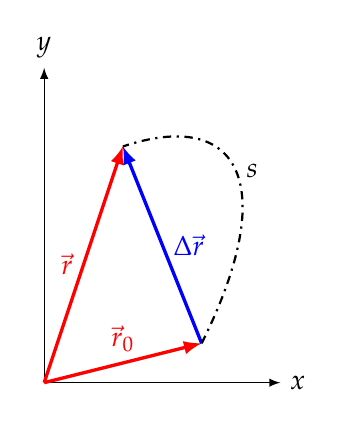
\begin{tikzpicture}[scale=.5]
      \draw[->](0,0)--(6,0) node[right]{$x$};
      \draw[->](0,0)--(0,8) node[above]{$y$};
      \draw[->,red,very thick] (0,0)--(4,1) node[midway,above]{$\vec r_0$};
      \draw[->,red,very thick] (0,0)--(2,6) node[midway,left]{$\vec r$};
      \draw[->,blue,very thick](4,1)--(2,6) node[midway,right]{$\Delta\vec r$};
      \draw[thick,dash dot] (4,1)..controls (6,5) and (5,7)..(2,6)
      node[midway,right]{$s$};
    \end{tikzpicture}
  \end{columns}
\end{frame}



\begin{frame}{Instantaneous \& Average Velocity}
  \textbf{Instantaneous velocity} $\vec v(t)$ is the rate of change of
  position\footnote{Or displacement} w.r.t.\ time. It is related to positiion
  $\vec r(t)$ by:

  \eq{-.13in}{
    \boxed{
      \vec v(t)= \diff{\vec r}t
      \quad\quad
      \vec r(t)=\int\vec v(t)\dl t + \vec r_0
    }
  }

  The constant of integration $\vec x_0$ evaluated at $t=0$. Likewise, the
  \textbf{average velocity} $\vec v_\text{avg}(t)$ is the displacement (change
  in position) $\Delta\vec r(t)$ over a finite time interval $\Delta t$:

  \eq{-.1in}{
    \boxed{
      \vec v_\text{avg}(t) = \frac{\Delta\vec r}t=
      \frac{\vec r(t)-\vec r_0}{\Delta t} = \frac{\int_0^t\vec v\dl t}{\Delta t}
    }
  }

  The SI unit of velocity is \textbf{meters per second} (\si{\metre\per\second})
  \vspace{.2in}
\end{frame}




\begin{frame}{Instantaneous \& Average Speed}
  \textbf{Instantaneous speed} $v$ is the time rate of change of
  \emph{distance}. It is the \emph{magnitude} of instantaneous velocity
  (i.e.\ $v=|\vec v|$). Since $s\geq 0$, instantaneous speed must be positive,
  i.e.\ $v\geq 0$.

  \eq{-.1in}{
    \boxed{
      v=\diff st \geq 0
    }
  }

  \textbf{Average speed} $v_\text{avg}(t)$ is the distance $s(t)$ travelled
  over a finite time interval $\Delta t$:
  
  \eq{-.1in}{
    \boxed{
      v_\text{avg}(t)=\frac{s(t)}{\Delta t}=\frac{\int_0^t v\dl t}{\Delta t}
    }
  }

  The SI unit of speed is also \si{\metre\per\second}.
\end{frame}



%\begin{frame}{Path}
%  Sometimes instead of explicitly describing the position $x=x(t)$ and $y=y(t)$,
%  the path of an object can be given in terms of $x$ coordinate $y=y(x)$, while
%  giving the $x$ (or $y$) coordinate as a function of time.
%  \begin{itemize}
%  \item In this case, substitute the expression for $x(t)$ into $y=y(x)$ to
%    get an expression of $y=y(t)$
%  \item Take derivative using chain rule to get $v_y=v_y(t)$
%  \end{itemize}
%\end{frame}


\begin{frame}{Instantaneous \& Average Acceleration}
  In the same way that velocity is the time rate of change in position,
  \textbf{instantaneous acceleration} $\vec a(t)$ is related to
  instantaneous velocity by:

  \eq{-.1in}{
    \boxed{
      \vec a(t)= \diff{\vec v}t=\diff[2]{\vec r}t
      \quad\quad
      \vec v(t)=\int\vec a(t)\dl t+\vec v_0
    }
  }

  The SI unit of velocity is \textbf{meters per second squared}
  (\si{\metre\per\second\squared}). \textbf{Average acceleration}
  $\vec a_\text{avg}(t)$ is the finite change in velocity $\Delta\vec v(t)$ over
  a finite time interval $t$:

  \eq{-.1in}{
    \boxed{
      \vec a_\text{avg}(t)=
      \frac{\Delta\vec v(t)}t
      =\frac{\vec v(t)-\vec v_0}t
      =\frac{\int_0^t\vec a\dl t}t
    }
  }

  Note that acceleration only requires a \emph{change} in velocity. It does
  \emph{not} necessarily mean an object speeds up or slows down (e.g.\ uniform
  circular motion).
\end{frame}



\begin{frame}{Special Notation When Differentiating With Time}
  Physicists and engineers often use a special notation when the derivative is
  taken with respect to \emph{time}, by writing a dot above the variable. For
  example:

  \vspace{-.3in}{\large
    \begin{align*}
      v &= \dot r \\
      a &= \dot v =\ddot r
    \end{align*}
  }

  We will use this notation whenever it is convenient
\end{frame}


\begin{frame}{Linear Independence}
  The $x$, $y$ and $z$ components of $\vec r$ along the $\iii$, $\jjj$ and
  $\kkk$ directions are \emph{linearly independent}, therefore the time
  derivative and integral can be separated into components:

  \vspace{-.3in}{\large
    \begin{align*}
      \vec v(t) &=
      \diff xt\iii + \diff yt\jjj + \diff zt\kkk = v_x\iii + v_y\jjj + v_z\kkk\\
      \vec a(t) &=
      \diff{v_x}t\iii + \diff{v_y}t\jjj + \diff{v_z}t\kkk =
      a_x\iii + a_y\jjj + a_z\kkk
    \end{align*}
  }
\end{frame}



\begin{frame}{If You Are Curious}
  The time derivative of acceleration is called \textbf{jerk}, with a unit
  of \si{\metre\per\second\cubed}:

  \eq{-.1in}{
    \vec j(t)=\diff{\vec a}t=\diff[2]{\vec v}t=\diff[3]{\vec r}t
  }

  The time derivative of jerk is \textbf{jounce}, or \textbf{snap}, with a
  unit of \si{\metre\per\second^4}:
  
  \eq{-.1in}{
    \vec s(t)=\diff{\vec j}t
    =\diff[2]{\vec a}t=\diff[3]{\vec v}t=\diff[4]{\vec r}t
  }
  
  The next two derivatives of snap are called \textbf{crackle} and
  \textbf{pop}, but these higher derivatives of position vector are rarely used.
  We will \emph{not} be using them.
\end{frame}



\begin{frame}{Acceleration as Functions of Velocity and Position}
  Acceleration may be expressed as functions of velocity and position rather
  than of time, if motion is driven by these forces:
  \begin{itemize}
  \item Gravitational or electrostatic forces:
    $a(r)=\dfrac{Gm_s}{r^2}\quad a(r)=\dfrac{kq_1q_2}{mr^2}$
  \item Spring force: $a(r)=-\dfrac kmr$
  \item Damping force: $a(v)=-bv$
  \item Aerodynamic lift and drag:
    $a(v)=\left[\dfrac{\rho C_L A}{2m}\right] v^2$ and
    $a(v)=\left[\dfrac{\rho C_D A}{2m}\right]v^2$
  \end{itemize}

  \vspace{.1in}In these cases, solving for $r(t)$, $v(t)$ and $a(t)$ will
  require solving a differential equation (see handout).
\end{frame}



\section{Kinematic Equations}

\begin{frame}{Kinematic Equations}
  While kinematic problems in AP Physics C exams often require calculus, these
  basic kinematic equations for \underline{constant acceleration} are still a
  powerful tool.

  \vspace{-.2in}{\large
    \begin{align*}
      x &= x_0+ v_0t + \frac12at^2\\
      v &= v_0+at\\
      v^2 &= v_0^2+ 2a(x-x_0)
    \end{align*}
  }

  For AP Physics, you will only be given three kinematic equations in your
  equation sheet. You will still be required to integrate when acceleration is
  not constant.
\end{frame}



\section{Motion Graphs}

\begin{frame}{Motion Graphs}
  You should already be familiar with the basic motion graphs for 1D motion:
  \begin{itemize}
  \item Position vs.\ time graph
  \item Velocity vs.\ time graph
  \item Acceleration vs.\ time graph
  \end{itemize}

  However, depending on the situation, it may be more useful to plot motion
  using other quantities as well.
\end{frame}



\begin{frame}{Uniform Motion: Constant Velocity}
  \begin{center}
    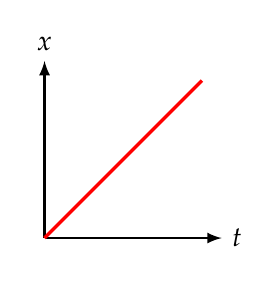
\begin{tikzpicture}[scale=.5]
      \draw[->,thick] (0,0)--(4.5,0) node[right]{$t$};
      \draw[->,thick] (0,0)--(0,4.5) node[above]{$x$};
      \draw[red,very thick](0,0)--(4,4);
    \end{tikzpicture}
    \hspace{.15in}
    \begin{tikzpicture}[scale=.5]
      \draw[->,thick] (0,0)--(4.5,0) node[right]{$t$};
      \draw[->,thick] (0,0)--(0,4.5) node[above]{$v$};
      \draw[red,very thick](0,2)--(4,2);
    \end{tikzpicture}
    \hspace{.15in}
    \begin{tikzpicture}[scale=.5]
      \draw[->,thick] (0,0)--(4.5,0) node[right]{$t$};
      \draw[->,thick] (0,0)--(0,4.5) node[above]{$a$};
      \draw[red,very thick](0,0)--(4,0);
    \end{tikzpicture}
  \end{center}
  \begin{itemize}
  \item Constant velocity has a straight line in the $x-t$ graph
  \item The slope of the $x-t$ graph is the velocity $v$, which is constant
  \item The slope of the $v-t$ graph is the acceleration $a$, which is zero in
    this case
  \end{itemize}
\end{frame}



\begin{frame}{Uniform Acceleration: Constant Acceleration}
  \begin{center}
    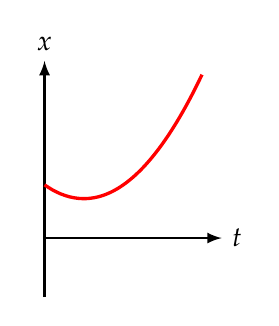
\begin{tikzpicture}[scale=.5]
      \draw[->,thick] (0,0)--(4.5,0) node[right]{$t$};
      \draw[->,thick] (0,-1.5)--(0,4.5) node[above]{$x$};
      \draw[smooth,samples=20,domain=0:4,red,very thick]
      plot({\x},{0.35*(\x-1)*(\x-1)+1});
    \end{tikzpicture}
    \hspace{.15in}
    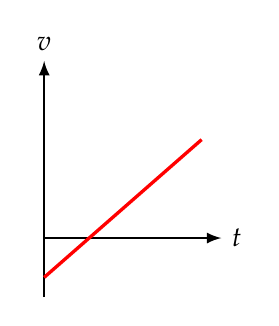
\begin{tikzpicture}[scale=.5]
      \draw[->,thick] (0,0)--(4.5,0) node[right]{$t$};
      \draw[->,thick] (0,-1.5)--(0,4.5) node[above]{$v$};
      \draw[red,very thick](0,-1)--(4,2.5);
    \end{tikzpicture}
    \hspace{.15in}
    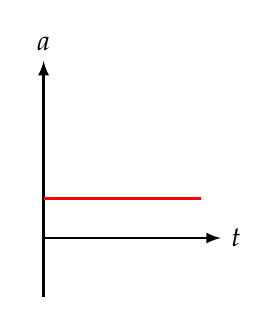
\begin{tikzpicture}[scale=.5]
      \draw[->,thick] (0,0)--(4.5,0) node[right]{$t$};
      \draw[->,thick] (0,-1.5)--(0,4.5) node[above]{$a$};
      \draw[red,very thick](0,1)--(4,1);
    \end{tikzpicture}
  \end{center}
  \begin{itemize}
  \item The $x-t$ graph for motion with constant acceleration is part of a
    \emph{parabola}
    \begin{itemize}
    \item If the parabola opens up, then acceleration is positive
    \item If the parabola opens down, then acceleration is negative
    \end{itemize}
  \item The $v-t$ graph is a straight line; its slope (a constant) is the
    acceleration
  \end{itemize}
\end{frame}



\begin{frame}{Simple Harmonic Motion}
  For \textbf{harmonic motions}, neither position, velocity nor acceleration
  are constant:

  \vspace{-.1in}
  \begin{center}
    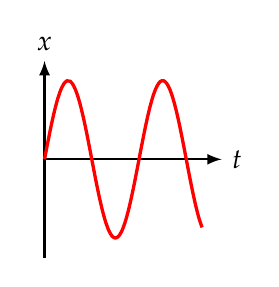
\begin{tikzpicture}[scale=.5]
      \draw[->,thick] (0,0)--(4.5,0) node[right]{$t$};
      \draw[->,thick] (0,-2.5)--(0,2.5) node[above]{$x$};
      \draw[smooth,samples=50,domain=0:4,red,very thick]
      plot({\x},{2*sin(150*\x)});
    \end{tikzpicture}
    \hspace{.15in}
    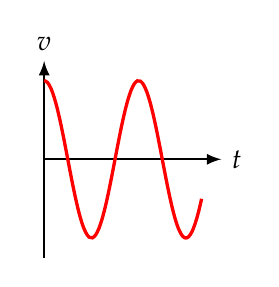
\begin{tikzpicture}[scale=.5]
      \draw[->,thick] (0,0)--(4.5,0) node[right]{$t$};
      \draw[->,thick] (0,-2.5)--(0,2.5) node[above]{$v$};
      \draw[smooth,samples=50,domain=0:4,red,very thick]
      plot({\x},{2*cos(150*\x)});
    \end{tikzpicture}
    \hspace{.15in}
    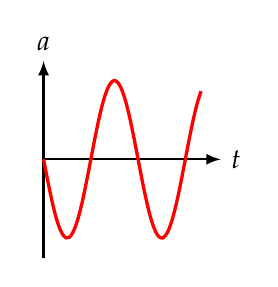
\begin{tikzpicture}[scale=.5]
      \draw[->,thick] (0,0)--(4.5,0) node[right]{$t$};
      \draw[->,thick] (0,-2.5)--(0,2.5) node[above]{$a$};
      \draw[smooth,samples=50,domain=0:4,red,very thick]
      plot({\x},{-2*sin(150*\x)});
    \end{tikzpicture}
  \end{center}
  Bottom line: regardless of the type motion,
  \begin{itemize}
  \item The $v-t$ graph is the slope of the $x-t$ graph
  \item The $a-t$ graph is the slope of the $v-t$ graph
  \end{itemize}
\end{frame}



\begin{frame}{Area Under Motion Graphs}
  \begin{columns}
    \column{.25\textwidth}
    \begin{center}
      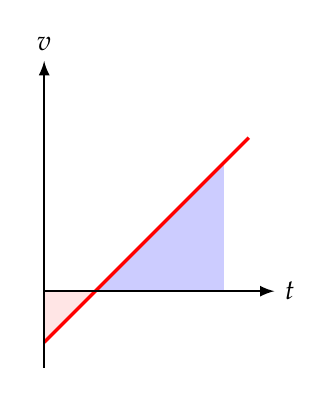
\begin{tikzpicture}[scale=.65]
        \draw[pink!40,fill=pink!40](0,0)--(0,-1)--(1,0)--cycle;
        \draw[blue!20,fill=blue!20](1,0)--(3.5,0)--(3.5,2.5)--cycle;
        \draw[red,very thick](0,-1)--(4,3);
        \draw[->,thick] (0,0)--(4.5,0) node[right]{$t$};
        \draw[->,thick] (0,-1.5)--(0,4.5) node[above]{$v$};
      \end{tikzpicture}
    \end{center}
    
    \column{.75\textwidth}
    The area under the $v-t$ graph is the displacement $x-x_0$.
    \begin{itemize}
    \item Area {\color{blue!20}\emph{above}} the time axis: $+$
      displacement
    \item Area {\color{red!40}\emph{below}} the time axis: $-$ displacement
    \end{itemize}
    \vspace{.2in}Likewise, the area under the $a-t$ graph is the change in
    velocity $v-v_0$.
  \end{columns}
\end{frame}



\begin{frame}{Velocity Squared vs.\ Displacement}
  If velocity information is given as a function of position\footnote{Depends
    on experimental set up} then a motion graph can be plotted using this
  kinematic equation:

  \eq{-.1in}{
    \underbracket{v^2}_y=\underbracket{v_0^2}_b+\underbracket{2a}_m
    \underbracket{(x-x_0)}_x
  }

  by plotting $v^2$ on the $y$-axis and displacement $\Delta x=x-x_0$ on the
  $x$-axis. The slope of the graph is $m=2a$. The square of the initial
  velocity ($v_0^2$) is the $y$-intercept.
\end{frame}



\begin{frame}{Graphing ``Linear'' Functions}
  This concept extends to graphing other physical quantities not relating to
  motion:
  \begin{itemize}
  \item To find the index of refraction of a material using Snell's law, plot
    $\sin\theta_i$ vs.\ $\sin\theta_2$ (rather than $\theta_1$ vs.\ $\theta_2$).
    The slope is the index $n$:

    \eq{-.1in}{
      \underbracket{\sin\theta_1}_y=\underbracket{n}_m
      \underbracket{\sin\theta_2}_x
    }
  \item To relate the period of oscillation of a simple pendulum to the length
    of the pendulum, plot $T^2$ vs.\ $L$:

    \eq{-.2in}{
      \underbracket{T^2}_y=\underbracket{\frac{4\pi^2}g}_m
      \underbracket{L}_x
    }
  \end{itemize}
\end{frame}



\section{Projectile Motion}

\begin{frame}{Projectile Motion}
  A \textbf{projectile} is an object that is launched with an initial velocity
  of $\vec v_0$ along a parabolic trajectory and accelerates only due to
  gravity.
  \begin{center}
    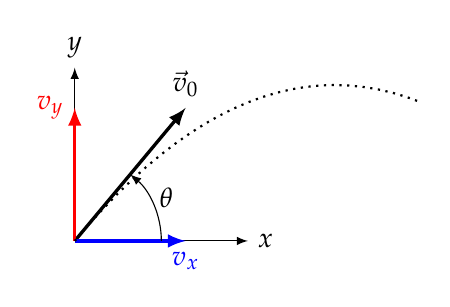
\begin{tikzpicture}[scale=1.1]
      \begin{scope}[->]
        \draw (0,0)--(2,0) node[right]{$x$};
        \draw (0,0)--(0,2) node[above]{$y$};
        \draw[very thick,rotate=atan(1.2)] (0,0)--(2,0)node[above]{$\vec v_0$};
        \draw[very thick,red] (0,0)--(0,2*sin{atan{1.2}}) node[left] {$v_y$};
        \draw[very thick,blue](0,0)--(2*cos{atan{1.2}},0) node[below]{$v_x$};
        \draw (1,0)arc(0:atan{1.2}:1) node[pos=.6,right]{$\theta$};
      \end{scope}
      \draw[dotted,domain=0:4,thick] plot (\x, {1.2*\x-.2*\x*\x});
    \end{tikzpicture}
  \end{center}
  \begin{itemize}
  \item $x$-axis is the \emph{horizontal} direction, with the ($+$) direction
    pointing \emph{forward}
  \item $y$-axis is the \emph{vertical} direction, with the ($+$) direction
    pointing \emph{up}
  \item The reference point is where the projectile is launched
  \item Consistent with the right-handed Cartesian coordinate system
  \item The launch angle $\theta$ is measured above the the horizontal.
  \end{itemize}
\end{frame}



\begin{frame}{Horizontal ($x$) Direction}
  There is no acceleration (i.e.\ $a_x=0$) along the horizontal direction,
  therefore horizontal velocity is constant. The kinematic equations reduce to:

  \eq{-.1in}{
    x(t)=v_xt=\left[v_0\cos\theta\right]t
  }

  where $x(t)$ is the horizontal position at time $t$, $v_0$ is the
  magnitude of the initial velocity, $v_x=v_0\cos\theta$ is its horizontal
  component.
\end{frame}




\begin{frame}{Vertical ($y$) Direction}
  Constant acceleration due to gravity alone along the vertical direction, i.e.\
  $a_y=-g$. (Acceleration is \emph{negative} due to the way we defined the
  coordinate system.) The important equation is this one:

  \eq{-.1in}{
    y(t) = \left[v_0\sin\theta\right]t-\frac12gt^2
  }

  These two kinematic equations may also be useful:

  \vspace{-.2in}{\large
    \begin{align*}
      v_y &= \left[v_0\sin\theta\right] -gt\\
      v_y^2&=\left[v_0\sin\theta\right]^2-2gy
    \end{align*}
  }
\end{frame}



\begin{frame}{Solving Projectile Motion Problems}
  Horizontal and vertical motions are independent of each other, but there are
  variables that are shared in both directions, namely:
  \begin{itemize}
  \item Time $t$
  \item Launch angle $\theta$ (above the horizontal)
  \item Initial speed $v_0$
  \end{itemize}
  
  \vspace{.2in}When solving any projectile motion problems
  \begin{itemize}
  \item \emph{Two} equations with \emph{two} unknowns
  \item If an object lands on an incline, there will be a third equation
    describing the relationship between $x$ and $y$
  \end{itemize}
\end{frame}



\begin{frame}{Symmetric Trajectory}
  A projectile's trajectory is symmetric if the object lands at the same height
  as when it launched. These equations are \emph{not} provided in the AP Exam
  equation sheet, but it can save you a lot of time if you can use them, instead
  of deriving them during the exam.
  \begin{itemize}
  \item Time of flight
    \eq{-.1in}{T=\frac{2v_0\sin\theta}g}
  \item Range
    \eq{-.1in}{R=\frac{v_0^2\sin(2\theta)}g}
  \item Maximum height
    \eq{-.1in}{H=\frac{v_0^2\sin^2\theta}{2g}}
  \end{itemize}
\end{frame}



\begin{frame}{Maximum Range}
  \eq{-.1in}{
    R=\frac{v_0^2\sin(2\theta)}g
  }
  
  \begin{itemize}
  \item Maximum range occurs at $\theta=\ang{45}$
  \item For a given initial speed $v_0$ and range $R$, launch angle $\theta$ is
    given by:
    
    \eq{-.1in}{
      \theta_1=\frac12\sin^{-1}\left(\frac{Rg}{v_0^2}\right)
    }

    But there is another angle that \emph{gives the same range}!

    \eq{-.1in}{
      \theta_2=\ang{90}-\theta_1
    }
  \end{itemize}
\end{frame}



\section{Relative Motion}

\begin{frame}{Relative Motion}
  
  \begin{block}{}
    \textbf{All motion quantities must be measured relative to a
      \emph{frame of reference}}
  \end{block}

  \vspace{.2in}
  \begin{itemize}
  \item\textbf{Frame of reference:} the \emph{coordinate system} from which all
    physical measurements are made.
  \item In \emph{classical} mechanics, the coordinate system is the
    Cartesian system
  \item There is no absolute motion/rest: all motions are relative
  \item\textbf{Principle of Relativity:} All laws of physics are equal in all
    inertial (non-accelerating) frames of reference
  \end{itemize}
\end{frame}  



\begin{frame}{Relative Motion}
  \begin{columns}
    \column{.4\textwidth}
    \begin{tikzpicture}[scale=1.3]
      \draw[->](0,0)--(-.5,-.5) node[left]{$x'$}
      node[pos=0,above left]{$\mathcal C$};
      \draw[->](0,0)--(1,0)     node[right]{$y'$};
      \draw[->](0,0)--(0,1)     node[above]{$z'$};

      \draw[->](2,3)--(1.5,2.5) node[left]{$x$}
      node[pos=0,above left]{$\mathcal B$};
      \draw[->](2,3)--(3,3)     node[right]{$y$};
      \draw[->](2,3)--(2,4)     node[above]{$z$};

      \fill[red] (3,1) circle(.03) node[right]{$A$};
    \end{tikzpicture}

    \column{.6\textwidth}
    Two frames of reference
    \begin{itemize}
    \item $\mathcal B$ with axes $x,y,z$
    \item $\mathcal C$ with axes $x',y',z'$
    \end{itemize}
    The two reference frames may (or may not) be moving relative to each other.
    The motion of the two reference frames affect how motion of
    $\color{red} A$ is calculated.
  \end{columns}
\end{frame}


\begin{frame}{Relative Motion}
  \begin{columns}
    \column{.4\textwidth}
    \begin{tikzpicture}[scale=1.3]
      \draw[->](0,0)--(-.5,-.5) node[left]{$x'$}
      node[pos=0,above left]{$\mathcal C$};
      \draw[->](0,0)--(1,0)     node[right]{$y'$};
      \draw[->](0,0)--(0,1)     node[above]{$z'$};

      \draw[->](2,3)--(1.5,2.5) node[left]{$x$}
      node[pos=0,above left]{$\mathcal B$};
      \draw[->](2,3)--(3,3)     node[right]{$y$};
      \draw[->](2,3)--(2,4)     node[above]{$z$};

      \draw[very thick,->,blue](0,0)--(3,1)  node[midway,below]{$\vec r_{AC}$};
      \draw[very thick,->,orange](2,3)--(3,1) node[midway,right]{$\vec r_{AB}$};
      \fill[red] (3,1) circle(.03) node[right]{$A$};
    \end{tikzpicture}

    \column{.6\textwidth}
    The position of $\color{red} A$ can be described by
    \begin{itemize}
    \item $\color{orange}\vec r_{AB}(t)$ (relative to frame $B$)
    \item $\color{blue}\vec r_{AC}(t)$ (relative to frame $C$)
    \end{itemize}
    It is obvious that $\color{orange}\vec r_{AB}(t)$ and
    $\color{blue}\vec r_{AC}(t)$ are different vectors
  \end{columns}
\end{frame}



\begin{frame}{Relative Motion}
  \begin{columns}
    \column{.4\textwidth}
    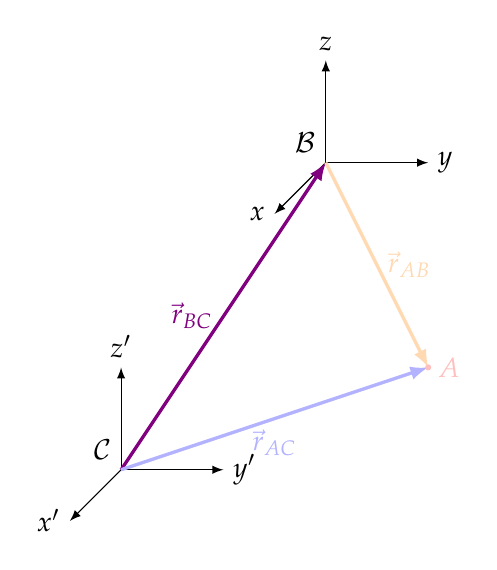
\begin{tikzpicture}[scale=1.3]
      \draw[->](0,0)--(-.5,-.5) node[left]{$x'$}
      node[pos=0,above left]{$\mathcal C$};
      \draw[->](0,0)--(1,0)     node[right]{$y'$};
      \draw[->](0,0)--(0,1)     node[above]{$z'$};

      \draw[->](2,3)--(1.5,2.5) node[left]{$x$}
      node[pos=0,above left]{$\mathcal B$};
      \draw[->](2,3)--(3,3)     node[right]{$y$};
      \draw[->](2,3)--(2,4)     node[above]{$z$};

      \begin{scope}[very thick,->] % vectors
        \draw[violet](0,0)--(2,3)  node[midway,left]{$\vec r_{BC}$};
        \draw[blue!30](0,0)--(3,1) node[midway,below]{$\vec r_{AC}$};
        \draw[orange!30](2,3)--(3,1)node[midway,right]{$\vec r_{AB}$};
      \end{scope}
      \fill[pink] (3,1) circle(.03) node[right]{$A$};
    \end{tikzpicture}

    \column{.6\textwidth}
    The position vector of the origins of the two reference frames is given by
    $\color{violet}\vec r_{BC}$
    \begin{itemize}
    \item The vector pointing from the origin of frame $C$ to the origin of
      frame $B$
    \item If the two frames are moving relative to each other, then
    $\color{violet}\vec r_{BC}$ is also a function of time
    \end{itemize}
    Even without using vector notations, the relationship between the vectors
    is obvious:

    \eq{-.1in}{
      \boxed{
        {\color{blue}\vec r_{AC}}=
        {\color{orange}\vec r_{AB}}+
        {\color{violet}\vec r_{BC}}
      }
    }
  \end{columns}
\end{frame}



\begin{frame}{Relative Motion}
  \begin{columns}
    \column{.4\textwidth}
    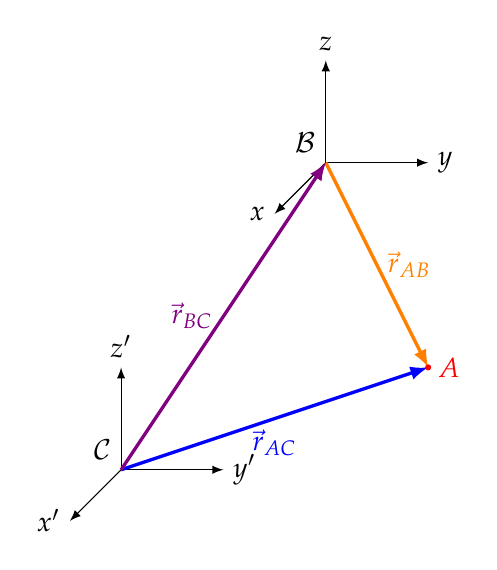
\begin{tikzpicture}[scale=1.3]
      \draw[->](0,0)--(-.5,-.5)  node[left]{$x'$}
      node[pos=0,above left]{$\mathcal C$};
      \draw[->](0,0)--(1,0) node[right]{$y'$};
      \draw[->](0,0)--(0,1) node[above]{$z'$};

      \draw[->](2,3)--(1.5,2.5)
      node[left]{$x$}
      node[pos=0,above left]{$\mathcal B$};
      \draw[->](2,3)--(3,3) node[right]{$y$};
      \draw[->](2,3)--(2,4) node[above]{$z$};

      \draw[very thick,->,blue](0,0)--(3,1)  node[midway,below]{$\vec r_{AC}$};
      \draw[very thick,->,orange](2,3)--(3,1) node[midway,right]{$\vec r_{AB}$};
      \draw[very thick,->,violet](0,0)--(2,3)node[midway,left] {$\vec r_{BC}$};
      \fill[red] (3,1) circle(.03) node[right]{$A$};
    \end{tikzpicture}

    \column{.6\textwidth}
    Starting from the definition of \textbf{relative position}:

    \eq{-.13in}{
      \boxed{
        {\color{blue}\vec r_{AC}} =
        {\color{orange}\vec r_{AB}} + {\color{violet}\vec r_{BC}}
      }
    }
    
    \vspace{-.13in}Differentiating all terms with respect to time, we get the
    equation for \textbf{relative velocity}:

    \eq{-.13in}{
      \boxed{
        {\color{blue}\vec v_{AC}} =
        {\color{orange}\vec v_{AB}}+ {\color{violet}\vec v_{BC}}
      }
    }

    \vspace{-.13in}Differentiating with respect to time again, and we obtain
    the equation for \textbf{relative acceleration}:

    \eq{-.13in}{
      \boxed{
        {\color{blue}\vec a_{AC}} =
        {\color{orange}\vec a_{AB}} + {\color{violet}\vec a_{BC}}
      }
    }
  \end{columns}
\end{frame}



\begin{frame}{Relative Velocity}
  In classical mechanics, the equation for relative velocities follows the
  \textbf{Galilean velocity addition rule}, which applies to speeds much less
  than the speed of light:

  \eq{-.1in}{
    \vec v_{AC}=\vec v_{AB}+\vec v_{BC}
  }

  The velocity of $A$ relative to reference frame $C$ is the velocity of $A$
  relative to reference frame $B$, plus the velocity of $B$ relative to $C$. If
  we add another reference frame $D$, the equation becomes:

  \eq{-.1in}{
    \vec v_{AD}=\vec v_{AB}+\vec v_{BC}+\vec v_{CD}
  }
\end{frame}



\begin{frame}{Typical Problems}
  In an AP Physics C exam, questions involving only kinematics usually appear
  in the multiple-choice section. The problems themselves are not very different
  compared to the Grade 12 Physics problems, but:
  \begin{itemize}
  \item You have to solve problems faster because of time constraint
  \item You can use $g=\SI{10}{\metre\per\second\squared}$
    in your calculations to make your lives simpler
  \item Many problems are \emph{symbolic}, which means that they deal with
    the equations, not actual numbers
  \item Will be coupled with other types (e.g.\ dynamics and rotational) in
    the free-response section
  \item You \emph{will} be given an equation sheet
  \end{itemize}
\end{frame}

\end{document}
